\documentclass[12pt,letterpaper]{article}

\usepackage[utf8]{inputenc}
\usepackage[T1]{fontenc}
\usepackage{amsmath}
\usepackage{amsfonts}
\usepackage{amssymb}
\usepackage{amsthm}
\usepackage[left=2cm,right=2cm,top=2cm,bottom=2cm,headheight=22pt]{geometry}
\usepackage{fancyhdr}
\usepackage{setspace}
\usepackage{lastpage}
\usepackage{graphicx}
\usepackage{caption}
\usepackage{subcaption}
\usepackage{paralist}
\usepackage{url}

\theoremstyle{definition}
\newtheorem{question}{Question}
\newtheorem{example}{Example}
\newtheorem{exercise}[question]{Exercise}
\newtheorem*{challenge}{Challenge}
\newtheorem*{theorem}{Theorem}
\newtheorem*{definition}{Definition}

\begin{document}

%Paramètres de mise en forme des paragraphes selon les normes françaises
\setlength{\parskip}{1ex plus 0.5ex minus 0.2ex}
\setlength{\parindent}{0pt}

%Paramètres relatifs aux en-têtes et pieds de page.
\pagestyle{fancy}
\lhead{Theron J Hitchman}
\chead{\Large Reading and Guided Practice \#03}
\rhead{Spring 2016}
\lfoot{\emph{Math and Decision Making }}
\cfoot{}
\rfoot{\emph{\thepage\ of \pageref{LastPage}}}

\section*{Introduction}

We will collect some new ideas that help us distinguish graphs as non-isomorphic. We will also conclude our
study of the Five Cities Puzzle by giving two proofs that it is impossible.

\section*{Goals}
At the end of this assignment, a student should be able to:
\begin{compactitem}
\item use the terms \emph{degree}, \emph{degree sequence}, \emph{cycle}, \emph{length of a cycle}, and \emph{tree} properly.
\item discuss the concept of an invariant.
\item State and use a theorem about the sum of the degrees of the vertices in a graph.
\end{compactitem}
A student might also be able to:
\begin{compactitem}
\item explain why the Five Cities Puzzle is unsolvable.
\item Give a proof that the graph $K_5$ has crossing number equal to $1$.
\item Settle the Three Utilities Puzzle.
\end{compactitem}

\section*{Reading and Questions for Graph Theory Meeting Four}

\subsection*{Invariants for Graphs}

We have now collected a whole list of interesting properties of graphs. Some of these properties are so integral
the the basic structure of a graph, that they are the same no matter how you draw the graph. Such a thing is
called an \emph{invariant} of the graph. What are some of these things? Let's make a list of a few we have previously discussed.
\begin{itemize}
\item The number of vertices.
\item The number of edges.
\item The number of components.
\end{itemize}

The main point of an invariant is that it helps you say for sure when two graphs are non-isomorphic. That is, it helps you say when two graphs are genuinely different. Can you see this for our examples? If two graphs are isomorphic, then the quantities above are the same for the two graphs.

So, if we have a pair of graphs and one of those quantities is \textit{different} between the two, then the graphs
cannot be isomorphic.

\begin{exercise}
Make a pair of graphs which are not isomorphic because they have a different number of vertices.
\end{exercise}

\begin{exercise}
Make a pair of graphs which have the same number of vertices, but which are not isomorphic because they 
have different numbers of edges.
\end{exercise}

\begin{exercise}
Make a pair of graphs which have the same number of vertices and the same number of edges, but which are 
not isomorphic because they have different numbers of components.
\end{exercise}

\subsection*{Degrees and the Degree Sequence}

Here is another invariant, which is at the next level of subtlety. Each vertex of a graph has a certain number of 
edges connected to it. The number of edges connected to a vertex is called the \emph{degree} of the vertex.
Our favorite graphs are distinguishable by looking at the degrees of their vertices.
\begin{figure}[h]
\centering
\begin{subfigure}[b]{.4\textwidth}
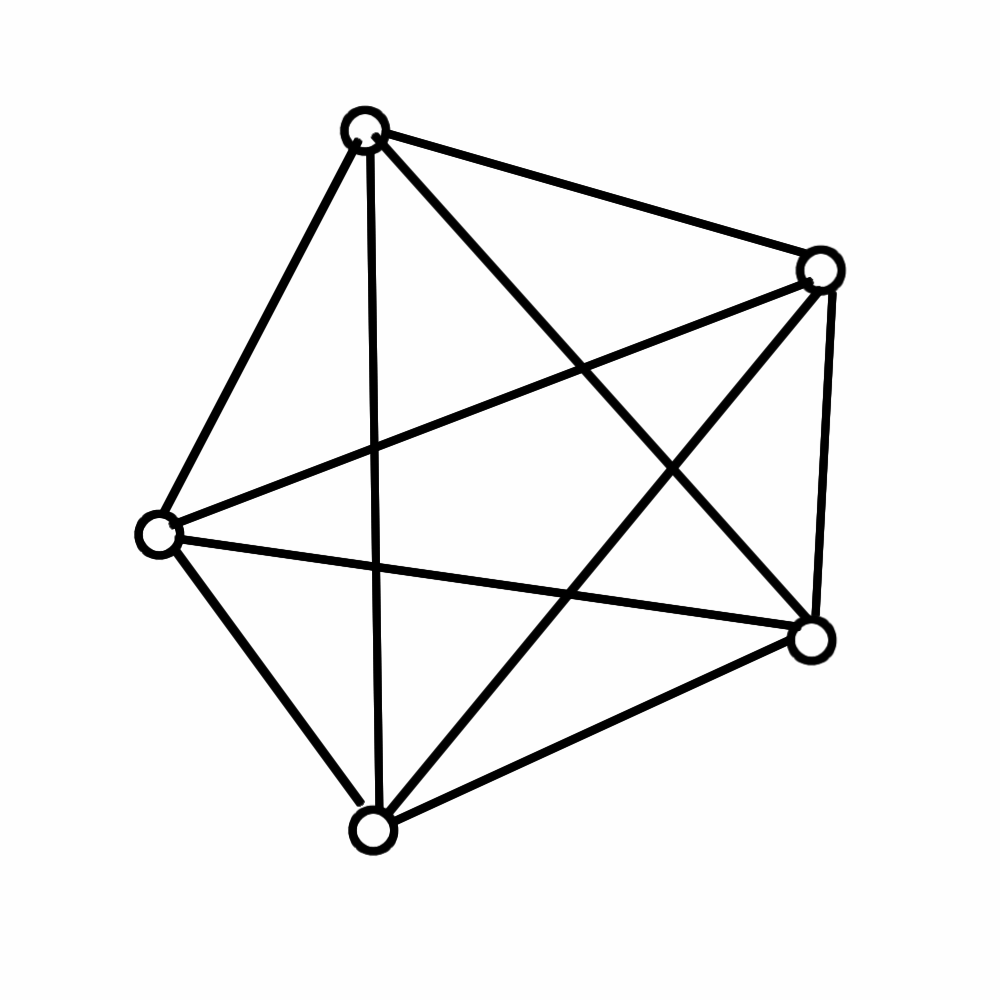
\includegraphics[width=\textwidth]{images/k5.png}
\caption{The graph $K_5$}
\label{figure:k5}
\end{subfigure}
\begin{subfigure}[b]{.4\textwidth}
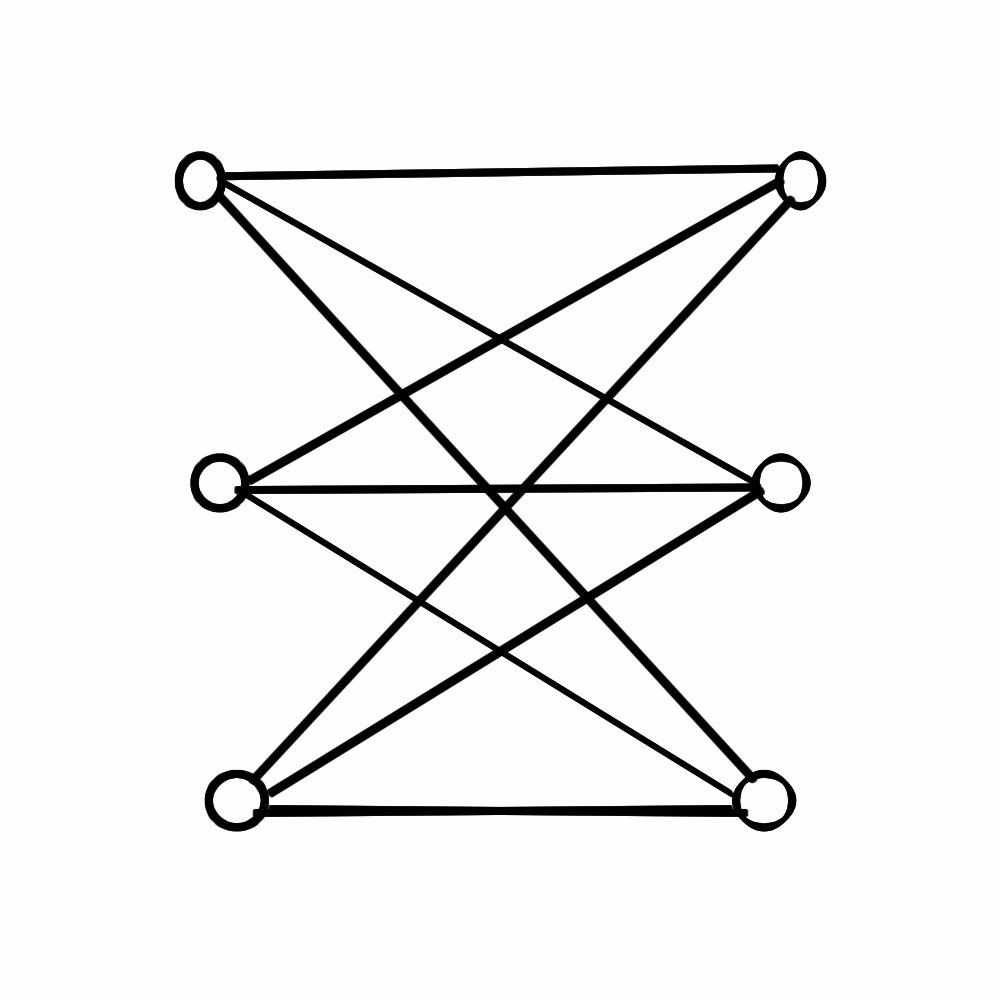
\includegraphics[width=\textwidth]{images/k3,3.png}
\caption{The graph $K_{3,3}$}
\label{figure:k33}
\end{subfigure}
\caption{Our Two Best Friends}
\label{figure:complete_graphs}
\end{figure}


\begin{exercise}
Check that $K_5$, the complete graph on five vertices, has every vertex of degree equal to $4$. 
\end{exercise}

\begin{exercise}
Check that $K_{3,3}$, the complete bipartite graph on three and three vertices, has every vertex of degree $3$.
\end{exercise}

%\begin{thebibliography}{9}
%\end{thebibliography}

\end{document}
%sagemathcloud={"zoom_width":100}























